\documentclass[tikz,border=5pt]{standalone}
\pdfinfoomitdate=1
\pdftrailerid{}
\pdfsuppressptexinfo=-1
\usepackage{pgfplots}
\usepgfplotslibrary{groupplots}
\pgfplotsset{compat=1.18}
\definecolor{atlas0}{HTML}{0072B2}
\definecolor{atlas1}{HTML}{E69F00}
\definecolor{atlas2}{HTML}{009E73}
\definecolor{atlas3}{HTML}{CC79A7}
\definecolor{atlas4}{HTML}{D55E00}
\definecolor{atlas5}{HTML}{56B4E9}
\definecolor{atlas6}{HTML}{000000}
\definecolor{atlas7}{HTML}{6A3D9A}
\definecolor{atlas8}{HTML}{A6CEE3}
\definecolor{atlas9}{HTML}{B2DF8A}
% ATLAS figure F10; data_sha256=17c7fc8bf55a25414baa049b03a154ac74af638e52e1d93e4cc39a8230ad80be
\begin{document}
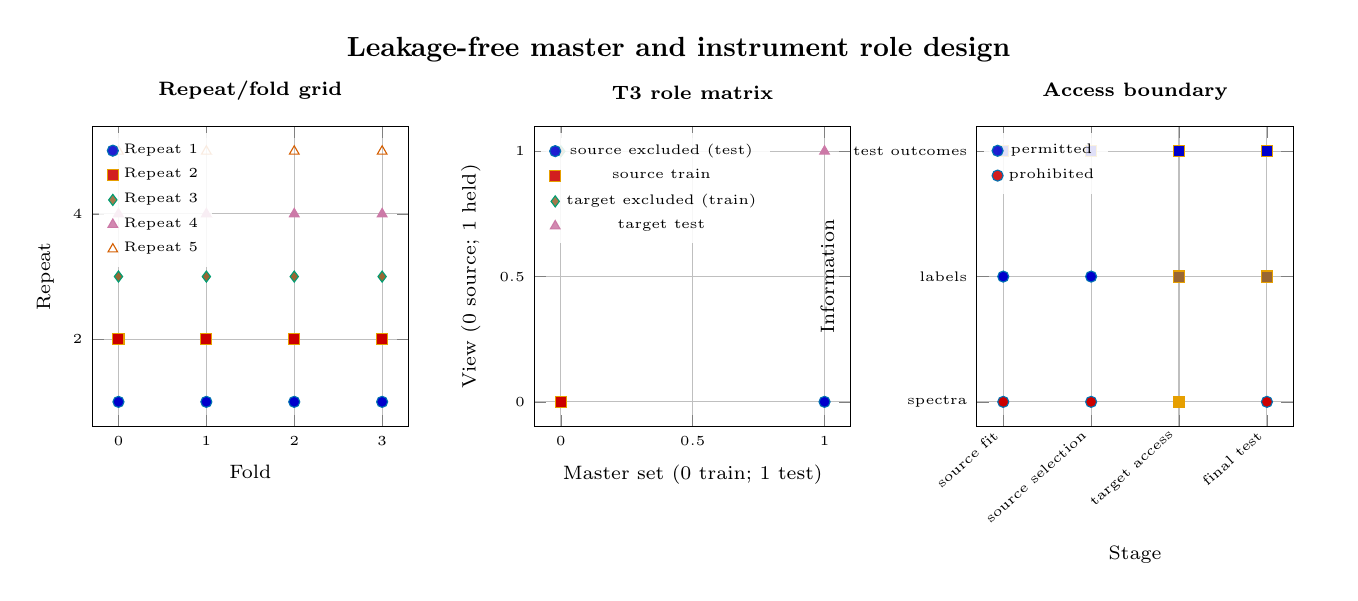
\begin{tikzpicture}
\begin{groupplot}[group style={group size=3 by 1, horizontal sep=1.6cm}, width=5.6cm, height=5.4cm, grid=major, tick label style={font=\tiny}, label style={font=\scriptsize}, title style={font=\scriptsize\bfseries,align=center,text width=4.7cm}, legend style={font=\tiny,draw=none,fill=white,fill opacity=0.88,text opacity=1,at={(0.02,0.98)},anchor=north west}]
\nextgroupplot[title={Repeat/fold grid},xlabel={Fold},ylabel={Repeat}]
\addplot+[only marks,color=atlas0,mark=*,mark size=2pt] coordinates {(0,1) (1,1) (2,1) (3,1)};
\addlegendentry{Repeat 1}
\addplot+[only marks,color=atlas1,mark=square*,mark size=2pt] coordinates {(0,2) (1,2) (2,2) (3,2)};
\addlegendentry{Repeat 2}
\addplot+[only marks,color=atlas2,mark=diamond*,mark size=2pt] coordinates {(0,3) (1,3) (2,3) (3,3)};
\addlegendentry{Repeat 3}
\addplot+[only marks,color=atlas3,mark=triangle*,mark size=2pt] coordinates {(0,4) (1,4) (2,4) (3,4)};
\addlegendentry{Repeat 4}
\addplot+[only marks,color=atlas4,mark=triangle,mark size=2pt] coordinates {(0,5) (1,5) (2,5) (3,5)};
\addlegendentry{Repeat 5}
\nextgroupplot[title={T3 role matrix},xlabel={Master set (0 train; 1 test)},ylabel={View (0 source; 1 held)}]
\addplot+[only marks,color=atlas0,mark=*,mark size=2pt] coordinates {(1,0)};
\addlegendentry{source excluded (test)}
\addplot+[only marks,color=atlas1,mark=square*,mark size=2pt] coordinates {(0,0)};
\addlegendentry{source train}
\addplot+[only marks,color=atlas2,mark=diamond*,mark size=2pt] coordinates {(0,1)};
\addlegendentry{target excluded (train)}
\addplot+[only marks,color=atlas3,mark=triangle*,mark size=2pt] coordinates {(1,1)};
\addlegendentry{target test}
\nextgroupplot[title={Access boundary},xlabel={Stage},ylabel={Information},xtick={0,1,2,3},xticklabels={source fit,source selection,target access,final test},x tick label style={rotate=42,anchor=east,font=\tiny},ytick={0,1,2},yticklabels={spectra,labels,test outcomes}]
\addplot+[only marks,color=atlas0,mark=*,mark size=2pt] coordinates {(0,1) (1,1)};
\addlegendentry{permitted}
\addplot+[only marks,color=atlas0,mark=*,mark size=2pt] coordinates {(0,0) (1,0) (3,0)};
\addplot+[only marks,color=atlas1,mark=square*,mark size=2pt] coordinates {(2,1) (3,1)};
\addlegendentry{prohibited}
\addplot+[only marks,color=atlas1,mark=square*,mark size=2pt] coordinates {(2,0)};
\addplot+[only marks,color=atlas1,mark=square*,mark size=2pt] coordinates {(0,2) (1,2) (2,2) (3,2)};
\end{groupplot}
\node[font=\normalsize\bfseries,anchor=south] at (current bounding box.north) {Leakage-free master and instrument role design};
\end{tikzpicture}
\end{document}
